\documentclass[a4paper,11pt]{article}
\usepackage[utf8]{inputenc}
\usepackage{graphicx}
\usepackage[hyphens]{url}
\usepackage[hidelinks]{hyperref}
\usepackage{tabularx}
\usepackage[centering, a4paper, margin=2.0cm, a4paper,]{geometry}
\usepackage[usenames,dvipsnames]{xcolor}
\usepackage{tikz} \usetikzlibrary{calc, arrows.meta, intersections, patterns, positioning, shapes.misc, fadings, through, decorations.pathreplacing}
\usepackage[utf8]{inputenc}
\usepackage{amsmath, amssymb, latexsym}
\usepackage{amsmath}
\usepackage{float}
\usepackage{eqexpl}
\eqexplSetDelim{=}
\eqexplSetIntro{where}
\usepackage{tikz}
\usetikzlibrary{decorations.pathreplacing}
\usetikzlibrary{fadings}
\usepackage{mathtools,amsfonts,amsthm}  % mathtools loads amsmath
\usepackage{placeins}
\usepackage{lipsum}

\definecolor{ColorOne}{named}{MidnightBlue}
\definecolor{ColorTwo}{named}{Dandelion}
\definecolor{ColorThree}{named}{Plum}
\definecolor{ColourFour}{named}{PineGreen}
\definecolor{ColourFive}{named}{OliveGreen}
%%%% modifying APS template a bit:
% times 
% \usepackage{mathptmx}
% arabic number section
% section left-side and title style
\usepackage{titlesec}
% spacing after and before section headers
\titlespacing*{\section}{0pt}{2.8ex plus 1ex minus .5ex}{2ex}
\titlespacing*{\subsection}{0pt}{2.2ex plus 1ex minus .5ex}{1.5ex}
\usepackage{natbib}
\definecolor{blueish2}{HTML}{0830Bb}
\hypersetup{colorlinks = true,
            linkcolor = blueish2,
            urlcolor  = blueish2,
            citecolor = black,
            anchorcolor = blueish2}
% section left-side and title style


\title{Borůvka's Algorithm}
% \author{NO AUTHORS GIVEN}
\author{Student Number: 700037512}
\date{Word count: 1214}


\begin{document}

\maketitle
\thispagestyle{empty}
\begin{abstract}
\noindent
Borůvka's Algorithm find a minimum spanning tree for a weighted undirected graph. It was the biginning of what is now a classic optimisation problem used in many fields. This report will discuss the algorithms main principles, complexity, successes, limitations and applications to explain why this particular algorithm changed the world.
\end{abstract}

\vspace*{\fill}
\begin{center}
\noindent I certify that all material in this report which is not my own work has been
identified
\end{center}
\vspace{1em}

Signature: \hrulefill
\clearpage
\pagenumbering{arabic} 

\newpage
\section{Introduction}
In 1926 Czech mathematician Otakar Borůvka published an algorithm to find the minimum spanning tree of a graph, in an attempt to optimise an electricity network for Moravia \cite{4392963}. It was the first algorithm of its kind and creating a minimum spanning tree has since become a classic optimisation problem with many different algorithmic solutions \cite{nevsetril2012origins}. A minimum spanning tree of a weighted, undirected graph $G(V,E)$, where V is the number of vertexes and E the number of edges, is the edges required to connect all the vertices for the lowest total edge cost without producing a cycle \cite{mst}. Figure 1 shows an example of a minimum spanning tree. 
\begin{figure}[!h]
    \centering
    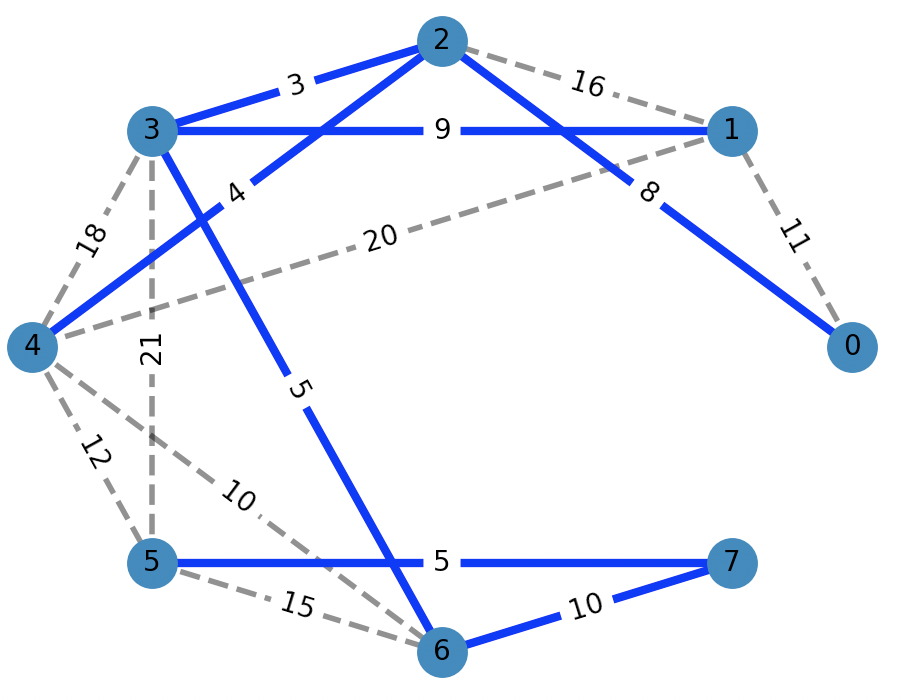
\includegraphics[width = 0.5\textwidth]{Screenshot 2022-12-07 at 5.26.26 pm.png}
    \caption{The minimum spanning tree created by Borůvka's Algorithm of the graph is shown in blue. It connects all nodes together and contains no cycles.}
    \label{fig:my_label}
\end{figure}
\FloatBarrier
Minimum spanning trees are used in a range of applications such as designing telecommunication and other digital networks \cite{nagarajan2014application}.
\section{Main Principles}

Borůvka's algorithm is a greedy algorithm, therefore, it selects the best option available at each step \cite{rachmawati2020comparative}. The input of the graph must be weighted such that all the edges have a corresponding cost, this can be physical distance, computational duration or anything that can numerically distinguish the cost of each path. Each edge must be undirected which means they can be traversed in either direction (a edge \verb|y| connecting \verb|a| and \verb|b| can be traversed from \verb|a| to \verb|b| or \verb|b| to \verb|a|). The algorithm begins setting all the nodes as separate components. The smallest connecting edge to every component is added to the minimum spanning tree and the nodes that have been connected merge into one component. This will create small disjoint trees where each tree signifies a component that must be connected together to form the minimum spanning tree. The process of finding the smallest connecting edge to each component continues until there is only one component containing all the nodes. The final remaining component is the minimum spanning tree. Figure 2 shows the process using a simple graph.
\begin{figure}[!h]
    \centering
    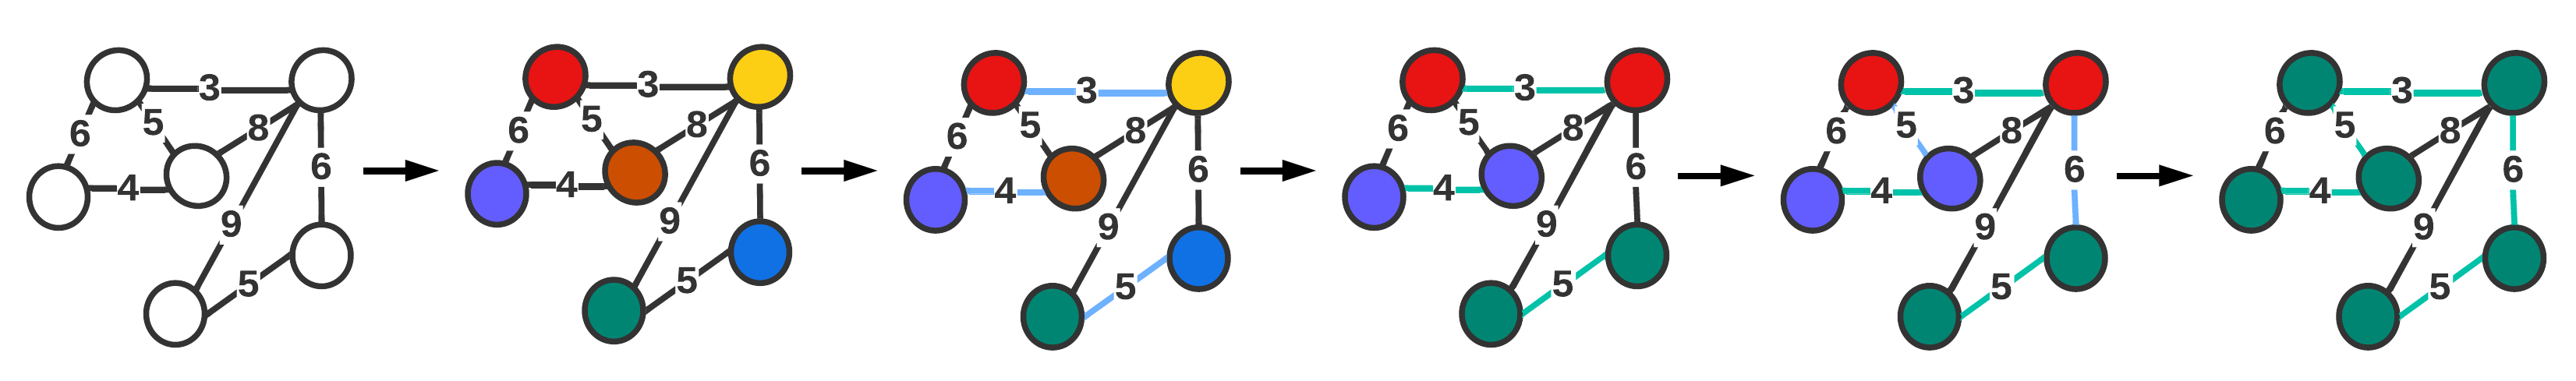
\includegraphics[width = \textwidth]{Gantt chart - Page 2 (3).png}
    \vspace{-3mm}
    \caption{Visual example of Borůvka's Algorithm. Each colour represents a component and the blue edges are the smallest edge connecting two components together at each step and form the minimum spanning tree.}
    \label{fig:my_label}
     \vspace{-3mm}
\end{figure}


\section{Pseudo code}
The Pseudo code for Borůvka's algorithm is given below. 

\begin{verbatim}
   1: def Borůvka's algorithm
        input: A undirected weighted graph G(V,E)
        output: The minimum spanning tree of G(V,E)
    
   2:   minimum_spanning_tree = []
   3:   component_size = []
   4:   for each vertex create a component containing only itself 
        and add 1 to the component_size list
   5:   no_components = number of vertices
   6:   while there is more than one component:
   7:       for every edge y connecting 2 components a and b in G:
   8:           let min_edge_a be the cheapest edge for a 
   9:           if y is smaller than min_edge_a:
  10:               min_edge_a <- y
  11:           let min_edge_b be the cheapest edge for b
  12:           if y is smaller than min_edge_b:
  13:               min_edge_b <- y
  14:       for every vertex in G:
  15:           if cheapest_edge for components is not null:
  16:               join the a and the b components together
  17:               add cheapest_edge to minimum_spanning_tree
  18:               no_components = no_components - 1
  19:   return(minimum_spanning_tree)
\end{verbatim}

\section{Complexity}
\subsection{Time Complexity}
The time complexity is $O(m\log(n))$ where $m$ is the number of edges and $n$ is the number of vertices \cite{FBAZLAMACCI2001767}. The outer while loop on line 6 in the pseudo code has time complexity $O(\log(n))$ because the loop halves the number of nodes each time so iterates $\log(n)$ times. The first inner for loop beginning on line 7 of the pseudo code is independent of the outer loop and has a time complexity of m because the algorithm looks at the edges each time. The second for loop beginning on line 14 has a time complexity of n as it iterates for the number of nodes. As such when the two inner nodes are added together the complexity is:

$O(m) + O(n) = O(max(m,n)) = O(m)$

assuming m > n which is the case if the graph has a cycle and therefore is not a minimum spanning tree. Hence the inner loops have a complexity of $O(m)$ which is iterated $O(\log(n))$ time giving the complexity of $O(m\log(n))$.

\subsection{Space Complexity}
The space complexity is $O(m + n)$ as the size of the input data is the size of the number of edges plus the number of nodes.
\section{Importance}
Borůvka algorithm helped advance the mathematical field of graph theory, shaping it into what it currently is in the present \cite{neuman199495}. His paper containing details of his minimum spanning tree algorithm was published 10 years before graph theory was officiated as a mathematical discipline. Graph theory has now expanded to include help solve problems such as image segmentation \cite{basavaprasad2014survey}, noting interactive chemical reactions \cite{gowda2021recent} and explaining sustainable supply chain networks \cite{luo2018explaining}.
 More directly, Borůvka's algorithm was cited in more recent minimum spanning tree algorithms, such as Kruskal's Algorithm \cite{kruskal1956shortest} then Prim's Algorithm \cite{prim1957shortest}. These algorithms are more commonly used than Borůvka's algorithm. Not only did the algorithm inspire others, but it has also been modified to reduce its time complexity and add parallelism \cite{7092783}. 
 
\section{Limitations}
 One limitation of the algorithm is that it is greedy which means in some cases the optimum solution is not found \cite{BANGJENSEN2004121}. This means earlier decisions are never reversed and if the local optimum is not the global optimum the algorithm will not alter the result to become globally optimum.
 However, this problem only occurs in a small fraction of graphs and the speed and reduced complexity using greedy algorithms are an acceptable trade-off in most circumstances.
 
 It is not used as commonly as Prim's or Kruskal's algorithm as it is more difficult to understand in comparison. The ability of non subject experts to understand the process is important when implementing programs across multiple fields such as biology or medical science \cite{loftus2022ideal}. 
The reason it is more difficult to understand can be turned into a strength because the structure can allow for parallelism which increases performance \cite{7092783}.
 
\section{Applications}
Borůvka's algorithm has possible applications in numerous areas, however, it has been optimised and commonly used in the areas discussed below.

An area which uses Borůvka's algorithm is image segmentation which can generate different scales of superpixels to identify elements or objects of a large image in real-time by turning the pixels into nodes \cite{basavaprasad2014survey}. These superpixels can then be used in machine learning. Its applications include ship detection and remote sensing.

Borůvka's algorithm is also used in wireless sensor networks to effectively distribute sensors as a grid which can be used for fire detection or art preservation \cite{chen2019coverage} \cite{ikikardes2006routing}.

Finally, the algorithm is used in reorganising databases so that the access time required to retrieve an object is minimised \cite{gabow1984scaling} \cite{wietrzyk1999dynamic}.

\section{Conclusion}
This algorithm changed the world by introducing an elegant solution to find the minimum spanning tree in a time complexity of $O(m\log(n))$. It inspired other such as Prim and Kruskal to do the same, advancing the area of graph theory. Despite some of its limitations it is still used today in various fields and has been modified to mitigate some of its previous drawbacks. 



\bibliographystyle{IEEEtran}
\bibliography{references}
\end{document}
